\documentclass[12pt,oneside,letterpaper,english]{article}
\usepackage[T1]{fontenc}
\usepackage[latin1]{inputenc}
\usepackage[margin=2.25cm,headheight=26pt,includeheadfoot]{geometry}
\usepackage[english]{babel}
\usepackage{listings}
\usepackage{color}
\usepackage{titlesec}
\usepackage{titling}
\usepackage[framed, numbered]{matlab-prettifier}
\usepackage{changepage}
\usepackage{amsmath}
\usepackage{hyperref}
\usepackage{enumitem}
\usepackage{graphicx}
\usepackage{fancyhdr}
\usepackage{lastpage}
\usepackage{caption}
\usepackage{tocloft}
\usepackage{setspace}
\usepackage{multirow}
\usepackage{titling}
\usepackage{float}
\usepackage{comment}
\usepackage{booktabs}
\usepackage{indentfirst}
\usepackage{lscape}
\usepackage{booktabs,caption}
\usepackage[flushleft]{threeparttable}
\usepackage[english]{nomencl}
\usepackage{xcolor}
\usepackage{lipsum}
\usepackage{datetime2}

% --- set footer and header ---
\pagestyle{fancy}
\fancyhf{}

\setlength{\parindent}{2em}
\title{Oscilloscope and Function generator} % to reference as \title, dont use \maketitle
\makeatletter\let\Title\@title\makeatother



\lstset{language=Matlab,
style=Matlab-editor,
basicstyle=\normalsize\mlttfamily,
numbers=left,
numberstyle={\scriptsize\color{black}},	% size of the numbers
numbersep=0.5cm											
}

\newlist{steps}{enumerate}{1}
\setlist[steps, 1]{leftmargin=1.5cm,label = Step \arabic*:}
\renewcommand{\headrulewidth}{1pt}
\renewcommand{\footrulewidth}{1pt}
\renewcommand{\rmdefault}{ptm}

%\lhead{\Title}
\rhead{\nouppercase{\rightmark}}
\lhead{\Title}
\rfoot{
\includegraphics[height=1.5cm]{root/Untitled.png}} % right header logo
\setlength\headheight{16pt}
\setlength{\footskip}{50pt}
\lhead{\Title} %rightH title
\cfoot{\thepage}

% --- End of page settings ---



\begin{document}
\pagenumbering{roman} 

\begin{titlepage}
\begin{center}
\vspace{2cm}
%\textsc{Oregon State University}\\[1.5cm]

\includegraphics[width=0.4\textwidth]{root/Untitled.png}~\\[2cm]
\vspace{2cm}

% Title
\hrule
\vspace{.5cm}
{ \huge \bfseries Oscilloscope and Function Generator} % title of the report
\vspace{.5cm}

\hrule
\vspace{1.5cm}

\textsc{\textbf{By}}\\
\vspace{.5cm}
\centering

% add your name here
K.Akhil - EE24BTECH11035\\
K.Teja Vardhan - EE24BTECH11034\\

\vspace{4cm}

\centering \today % see latexmkrc for time zone change
\end{center}
\end{titlepage}

\newpage
\doublespacing
%\addcontentsline{toc}{section}{Table of Contents}
\renewcommand{\baselinestretch}{1}\normalsize
\tableofcontents
\renewcommand{\baselinestretch}{1}\normalsize
%\singlespacing
\thispagestyle{fancy} % force page style

\newpage
\pagenumbering{arabic} 
\fancyfoot[C]{Page \thepage\ of \pageref{EndOfText}}
\section{Oscilloscope} \label{ch1}

An oscilloscope is an electronic instrument used to visualize and analyze electrical signals by displaying their voltage waveforms over time. It provides real-time information about the behavior of a signal, enabling users to measure parameters like amplitude, frequency, and waveform shape, which are crucial in various fields like electronics, telecommunications, and research.

\begin{figure}[h!]
    \centering
    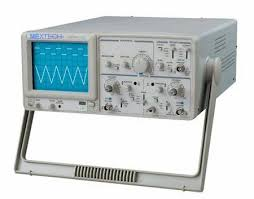
\includegraphics[width=0.4\textwidth]{figures/oscilloscope.jpeg}
    \caption{oscilloscope}
    \label{fig:sample_image}
\end{figure}
 

\subsection{How an Analog oscilloscope works?}
\begin{figure}[h!]
    \centering
    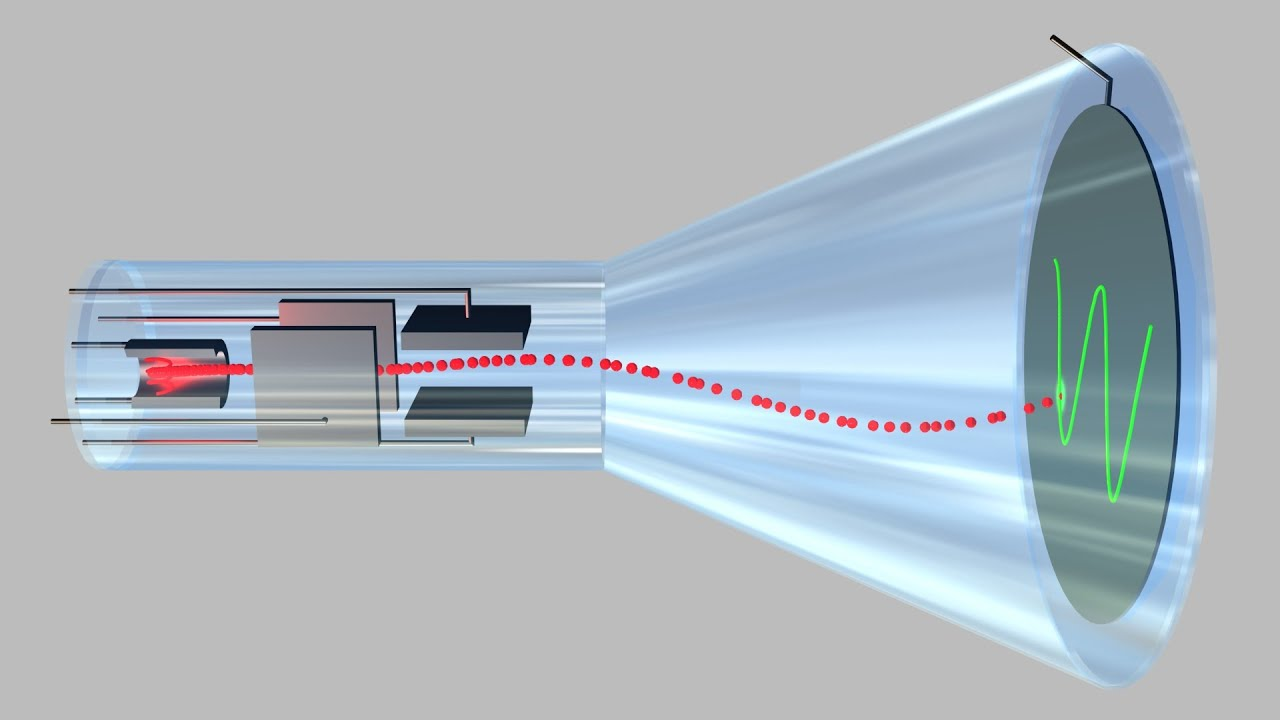
\includegraphics[width=0.4\textwidth]{figures/cathoderay.jpeg}
    \caption{This is a sample image.}
    \label{fig:sample_image}
\end{figure}

An analog oscilloscope uses an electron gun to direct a beam onto a phosphor-coated screen, where voltage waveforms are displayed. The vertical deflection plates control the beam's movement according to the input signal's voltage, and the horizontal deflection plates control the beam's movement based on time. The time base synchronizes the beam's horizontal sweep to ensure stable display. The signal's variations are shown as a trace on the screen, where each division corresponds to specific voltage or time intervals. Triggering ensures the waveform is stable and consistent.
\\

\subsection{How is Digital Oscilloscope Different from Analog Oscilloscope?}

Unlike an analog oscilloscope, a digital oscilloscope converts the analog input signal into digital data using an analog-to-digital converter (ADC). This digital representation is processed and displayed, providing more accuracy, stability, and flexibility. Digital oscilloscopes offer higher resolution, advanced triggering features, and the ability to store and recall waveforms for later analysis. They are generally more versatile, allowing for complex measurements and data manipulation, which makes them superior for detailed analysis compared to analog oscilloscopes.
 
\label{EndOfText}


\pagenumbering{arabic} 
\fancyfoot[C]{Page \thepage\ of \pageref{EndOfText}}
\section{Function Generator} \label{ch1}
\
A \textbf{function generator} is an electronic device used to generate various types of electrical waveforms over a wide range of frequencies. It is commonly used in electronics testing, development, and troubleshooting.

\begin{figure}[h!]
    \centering
    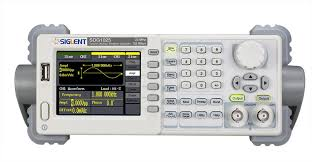
\includegraphics[width=0.6\textwidth]{figures/functiongenerator.jpeg}
    \caption{Function Generator}
    \label{fig:sample_image}
\end{figure}
\subsection{Key Features of a Function Generator}
\begin{itemize}
    \item \textbf{Waveform Types:}
    \begin{itemize}
        \item \textit{Sine wave:} Smooth periodic oscillations.
        \item \textit{Square wave:} Alternates between high and low levels, used in digital circuits.
        \item \textit{Triangle wave:} Linear rise and fall, used in modulation and testing.
        \item \textit{Sawtooth wave:} Sharp rise and slow fall or vice versa.
        \item \textit{Pulse wave:} Short-duration signal for timing and control purposes.\\
    \end{itemize}
    \item \textbf{Frequency Range:} Typically operates over a range from a few Hz to several MHz.
    \item \textbf{Amplitude Control:} Users can adjust the output signal's amplitude.
    \item \textbf{DC Offset:} Allows adding a constant voltage to the waveform.
    \item \textbf{Modulation:} Some function generators can apply modulation techniques like AM (Amplitude Modulation) or FM (Frequency Modulation).
    \item \textbf{Output Impedance:} Generally 50 ohms, matching typical test equipment.
\end{itemize}
\subsection{Applications}
\begin{itemize}
    \item \textbf{Testing Circuits:} Used to test amplifiers, filters, and other electronic circuits.
    \item \textbf{Signal Injection:} Provides input signals for troubleshooting and diagnostics.
    \item \textbf{Waveform Generation:} Generates waveforms for experimentation in labs.
    \item \textbf{Modulation and Timing:} Helps simulate signals for communication systems.
\end{itemize}

In advanced setups, function generators are often replaced by \textbf{arbitrary waveform generators (AWGs)} for more complex signal requirements.
 
\label{EndOfText}
\newpage
\pagenumbering{arabic} 
\fancyfoot[C]{Page \thepage\ of \pageref{EndOfText}}
\section{Lissajous Figures} \label{ch1}
Lissajous figures are intricate patterns that appear on an oscilloscope when two periodic signals-often sinusoidal but also including square or triangular waves-are displayed simultaneously on the horizontal and vertical axes. Named after physicist Jules Antoine Lissajous, these figures visually represent the relationship between the frequencies and phase differences of the signals. The resulting pattern varies depending on the frequency ratio, phase shift, and waveform type. While sinusoidal waveforms typically produce smooth, predictable patterns, other waveforms like square or triangular waves can create more complex or sharper figures. Lissajous figures serve as valuable tools for analyzing signal relationships in various applications, including frequency measurement and phase analysis.

\subsection{Some Examples and their Mathematical proofs}
\begin{enumerate}
\item \textbf{\large \textbf{$x = A_0 si(\omega t)$} and \textbf{$y = A_0 sin(\omega t )$}},
\begin{figure}[h!]
    \centering
    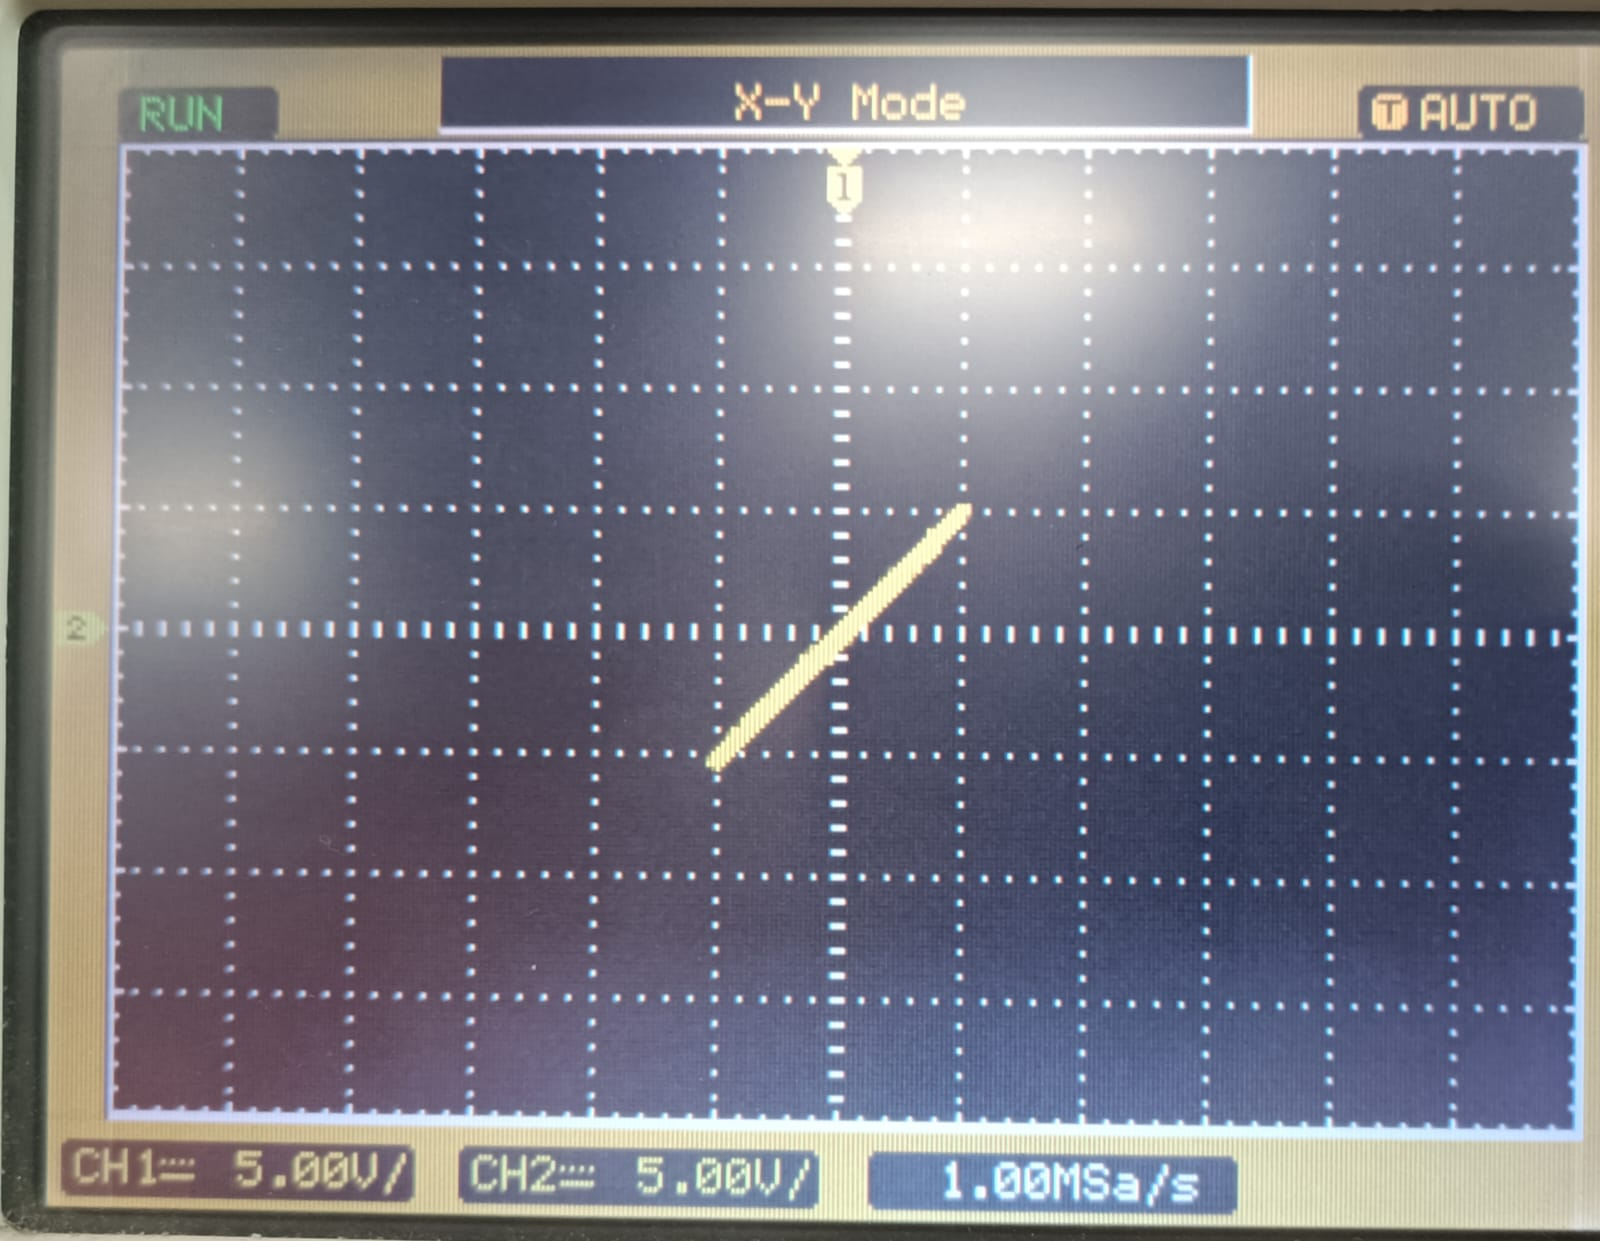
\includegraphics[width=0.6\textwidth]{actualgraph/line.jpeg}
    
    \caption{Graph of above signal using  Oscilloscope}
    \label{fig:sample_image}
    \end{figure}

    Mathematical proof,\\
    \[
    x=\sin(\omega t)
    \]
    \[
    y=\sin(\omega t )
    \]
    Now we can say , that \\
    $x=y$\\
    Therefore, it forms a straight line passing through origin and have slope 1.
    \begin{figure}[h!]
    \centering
    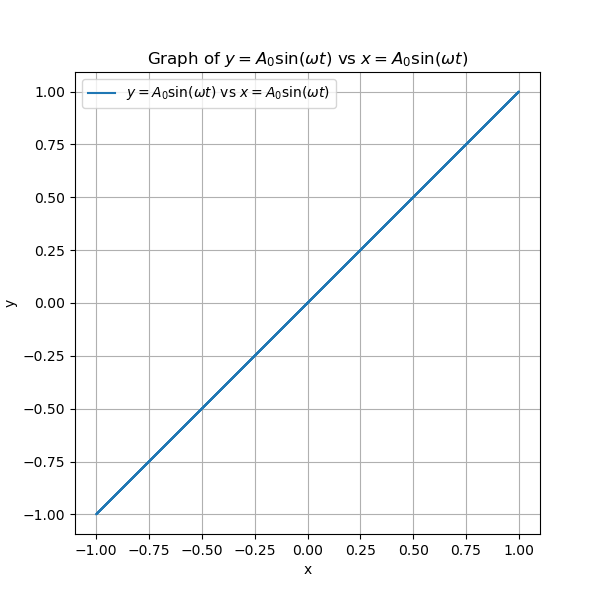
\includegraphics[width=0.6\textwidth]{graphs/Figure_2.png}
    \caption{Graph of above signal using python}
    \label{fig:sample_image}
     \end{figure}





\item   \textbf{\large \textbf{$x = A_0 sin(\omega t)$} and \textbf{$y = A_0 sin(\omega t + \frac{\pi}{2})$}},
    \begin{figure}[h!]
    \centering
    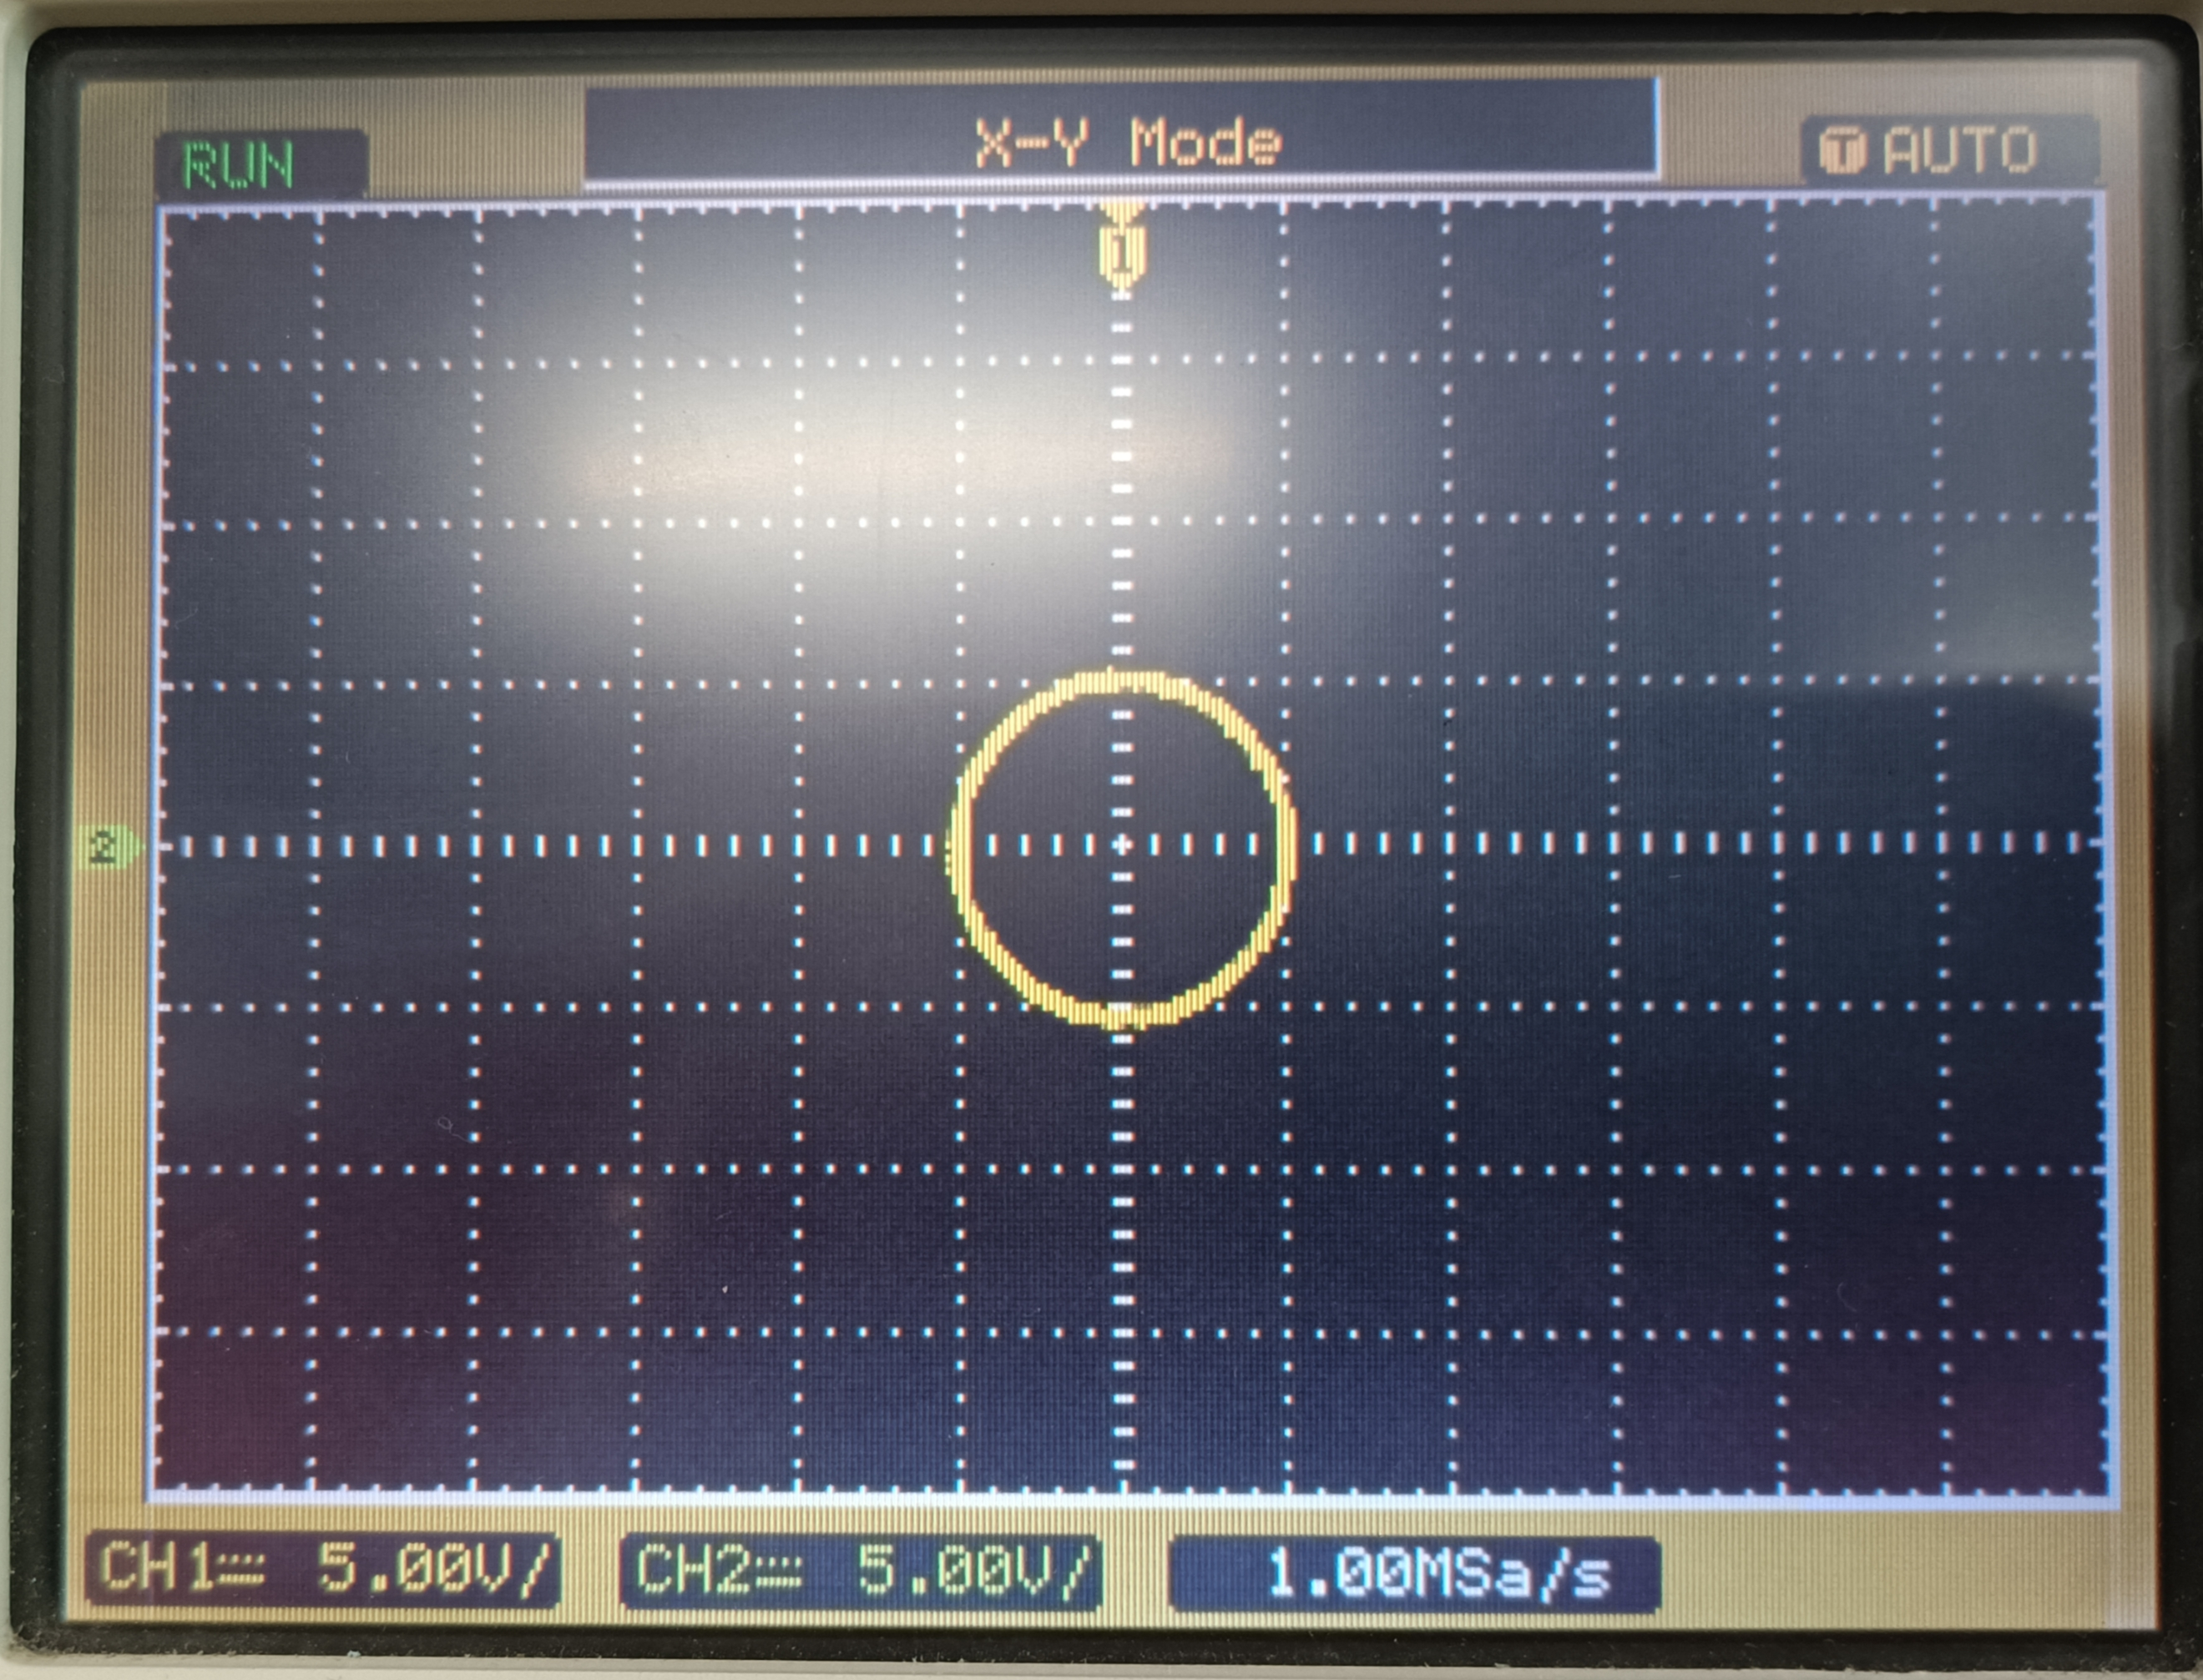
\includegraphics[width=0.6\textwidth]{actualgraph/circle.jpg}
    
    \caption{Graph of above signal using  Oscilloscope}
    \label{fig:sample_image}
    \end{figure}
(Here, Value of $\omega=2\pi 200$Hz)\\
Mathematical proof,\\
  \\ We consider two traveling waves with the same amplitude, frequency, and wavenumber but with a phase difference of \(90^\circ\):
\[
x(t) = A \sin(kx - \omega t) \quad \text{(wave along the \(x\)-axis)},
\]
\[
y(t) = A \sin\left(kx - \omega t + \frac{\pi}{2}\right) \quad \text{(wave along the \(y\)-axis)}.
\]
Using the trigonometric identity:
\[
\sin\left(kx - \omega t + \frac{\pi}{2}\right) = \cos(kx - \omega t),
\]
the equations become:
\[
x(t) = A \sin(kx - \omega t), \quad y(t) = A \cos(kx - \omega t).
\]
Resultant Curve,\\
To find the resultant curve, we eliminate \(t\) from the parametric equations. Using the Pythagorean identity:
\[
\sin^2\theta + \cos^2\theta = 1,
\]
we have:
\[
x^2 + y^2 = A^2 \sin^2(kx - \omega t) + A^2 \cos^2(kx - \omega t) = A^2.
\]
This is the equation of a \textbf{circle} with radius \(A\).

\begin{figure}[h!]
    \centering
    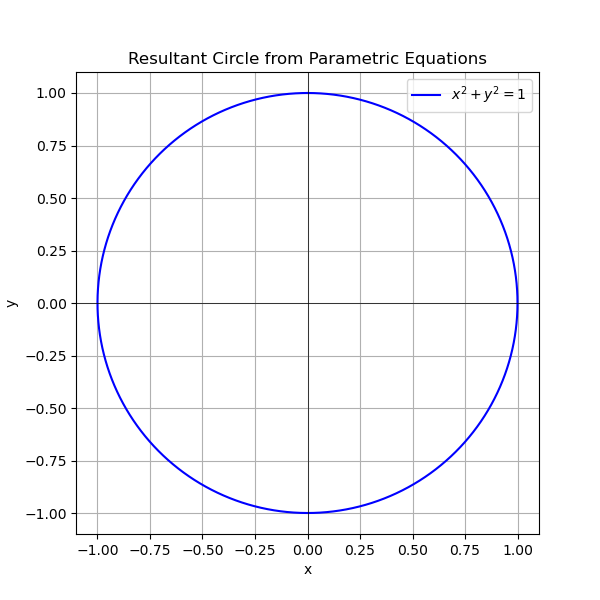
\includegraphics[width=0.3\textwidth]{graphs/1.png}
    \caption{Graph of above signal using python}
    \label{fig:sample_image}
     \end{figure}



\newpage
     
\item \textbf{\large \textbf{$x = A_0 sin(\omega t)$} and \textbf{$y = A_0 sin(\omega t + \frac{\pi}{4})$}},\\
     \begin{figure}[h!]
    \centering
    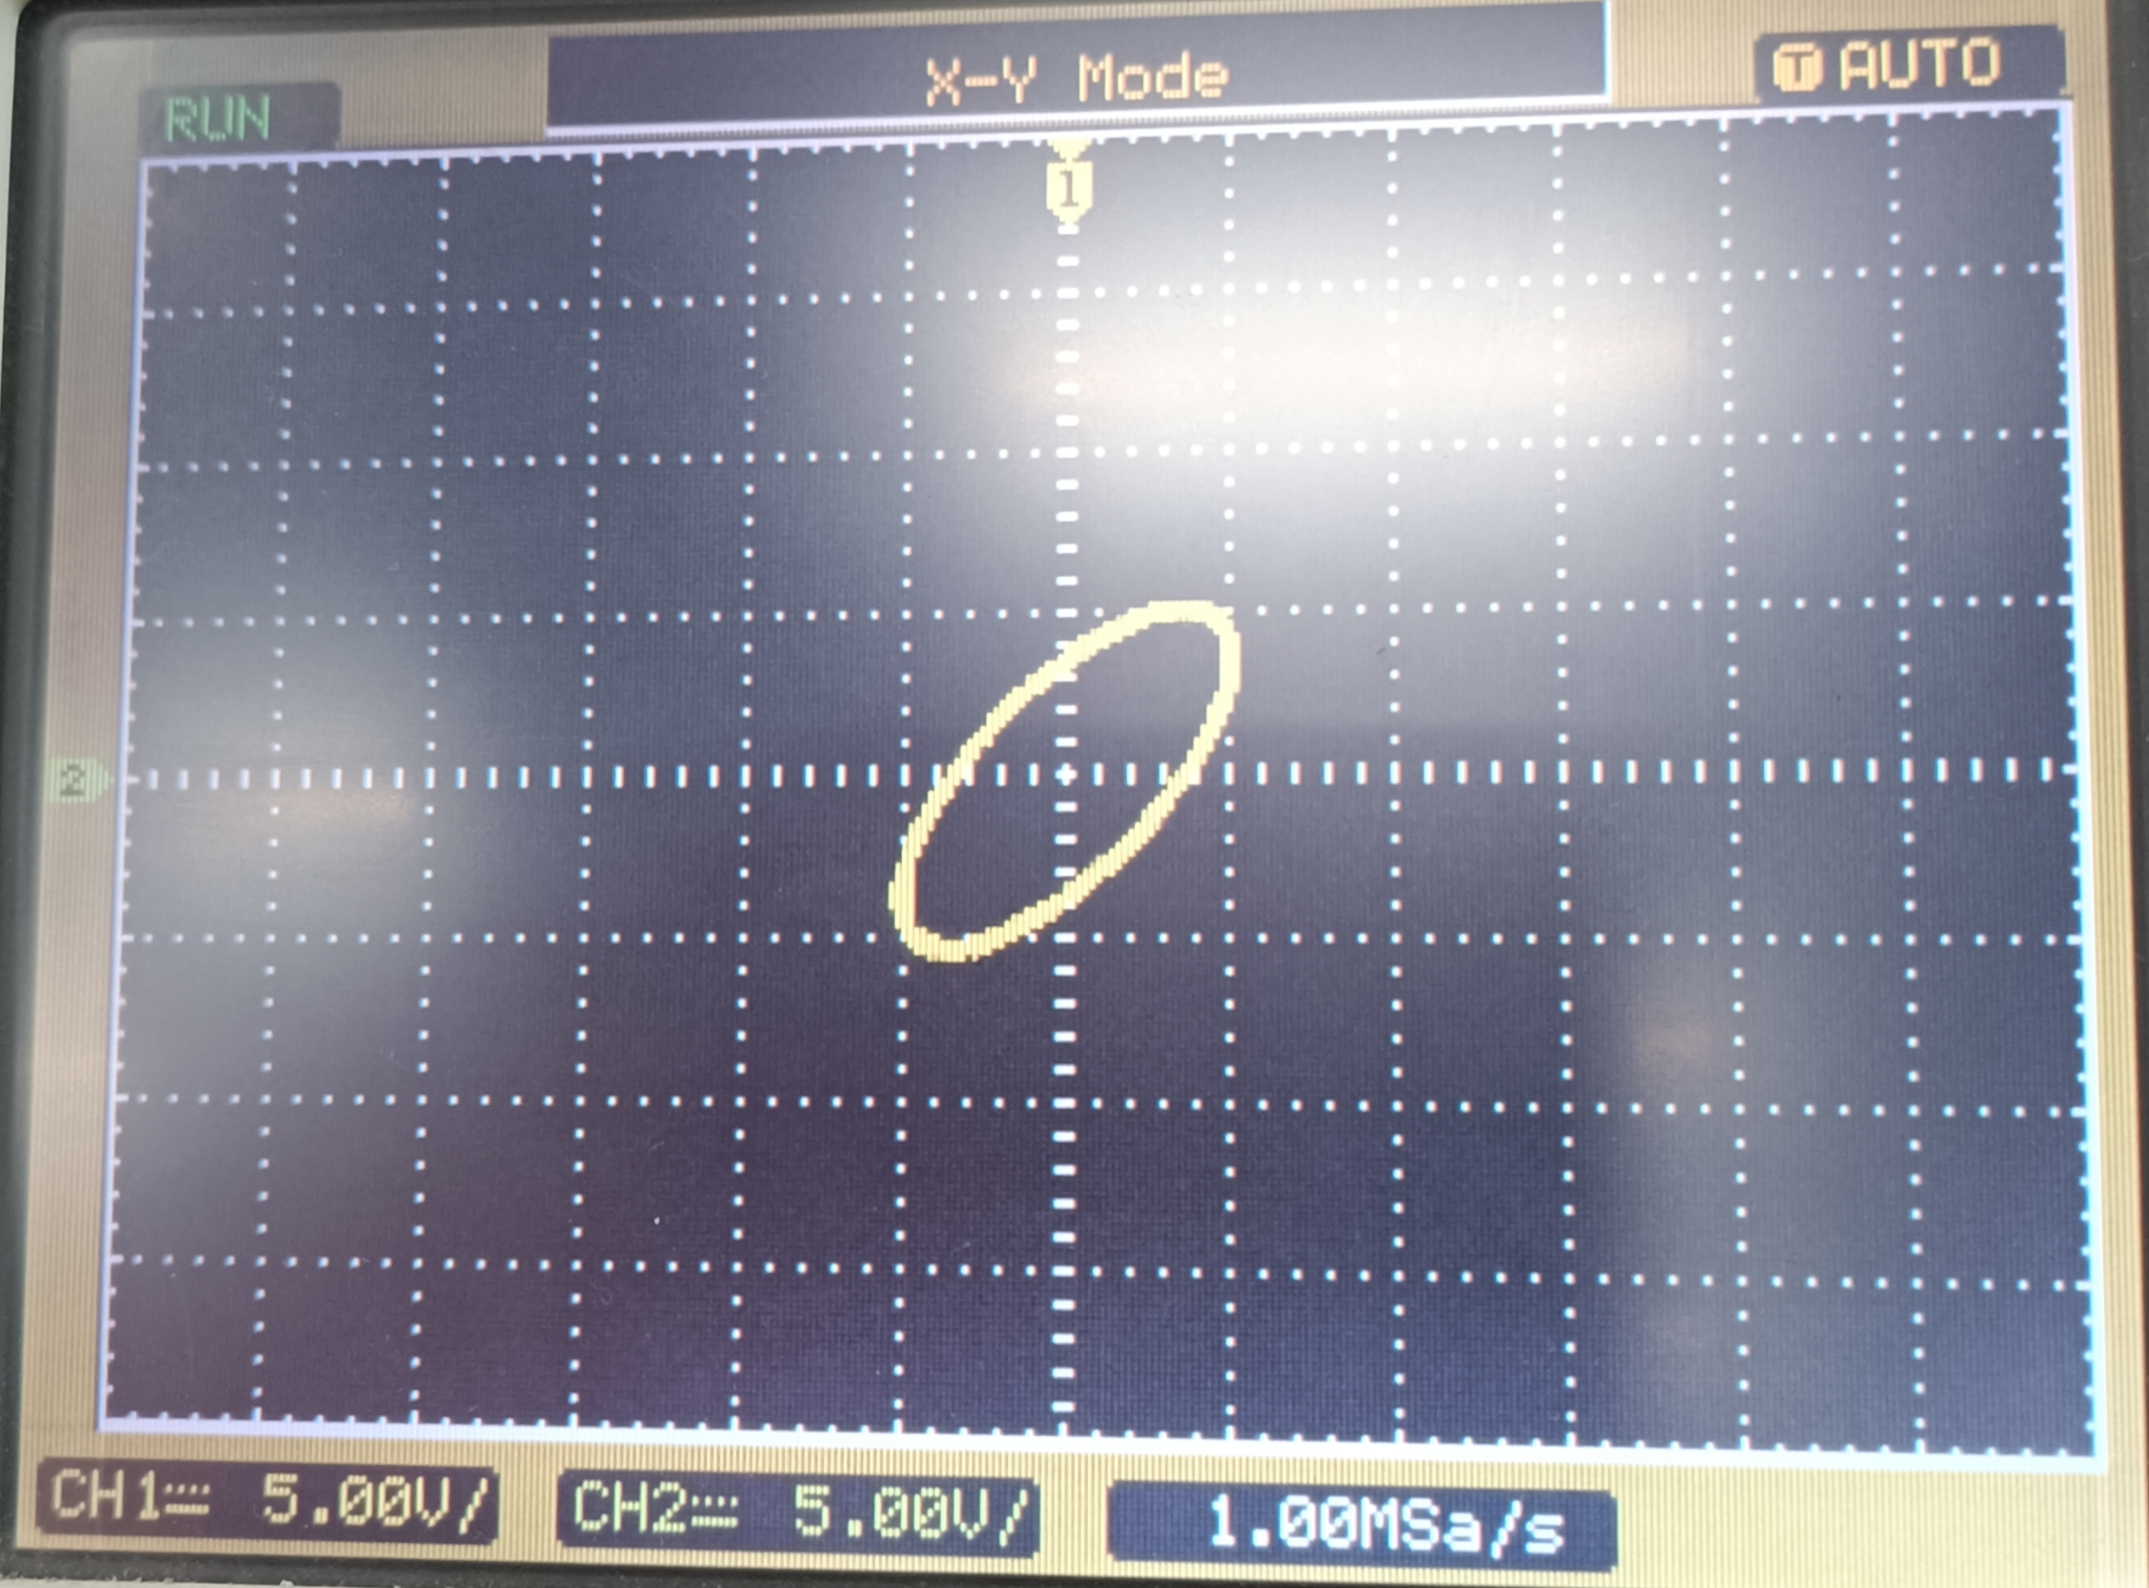
\includegraphics[width=0.6\textwidth]{actualgraph/ellipse.jpg}
    \caption{Graph of above signal using  Oscilloscope}
    \label{fig:sample_image}
    \end{figure}
Mathematical proof,\\
Express \( y \) in terms of \( x \),\\
We begin by rewriting the second equation for \( y \):
\[
y = A_0 \sin\left(\omega t + \frac{\pi}{4}\right)
\]
Using the trigonometric identity for \( \sin(A + B) \):
\[
\sin(A + B) = \sin A \cos B + \cos A \sin B,
\]
we get:
\[
y = A_0 \left[\sin(\omega t) \cos\left(\frac{\pi}{4}\right) + \cos(\omega t) \sin\left(\frac{\pi}{4}\right)\right]
\]
Since \( \cos\left(\frac{\pi}{4}\right) = \sin\left(\frac{\pi}{4}\right) = \frac{\sqrt{2}}{2} \), this simplifies to:
\[
y = A_0 \left[\frac{\sqrt{2}}{2} \sin(\omega t) + \frac{\sqrt{2}}{2} \cos(\omega t)\right]
\]
Now, using the first equation \( \sin(\omega t) = \frac{x}{A_0} \), we substitute into the above expression:
\[
y = \frac{A_0 \sqrt{2}}{2} \left( \frac{x}{A_0} + \cos(\omega t) \right)
\]
\[
y=\frac{1}{\sqrt{2}}x+\cos(\omega t)
\]
\[
y-\frac{1}{\sqrt{2}}x=\cos(\omega t)\frac{1}{\sqrt{2}}
\]
Squaring on Both sides,\\
\[
2y^2+x^2-2\sqrt{2}xy={A_0}^2-x^2
\]
\[
x^2+y^2+\sqrt{2}xy={A_0}^2
\]
Therefore, it is an ellipse.
  \begin{figure}[h!]
    \centering
    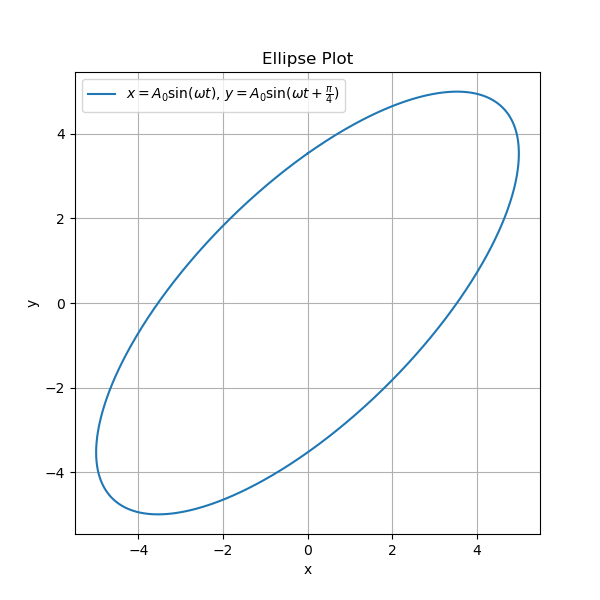
\includegraphics[width=0.4\textwidth]{graphs/Figure_1.png}
    \caption{Graph of above signal using python code}
    \label{fig:sample_image}
    \end{figure}








\newpage
\item \textbf{\large \textbf{$x = A_0 \sin(\omega t)$} and \textbf{$y = A_0 \sin(2\omega t)$}},
\begin{figure}[h!]
\centering
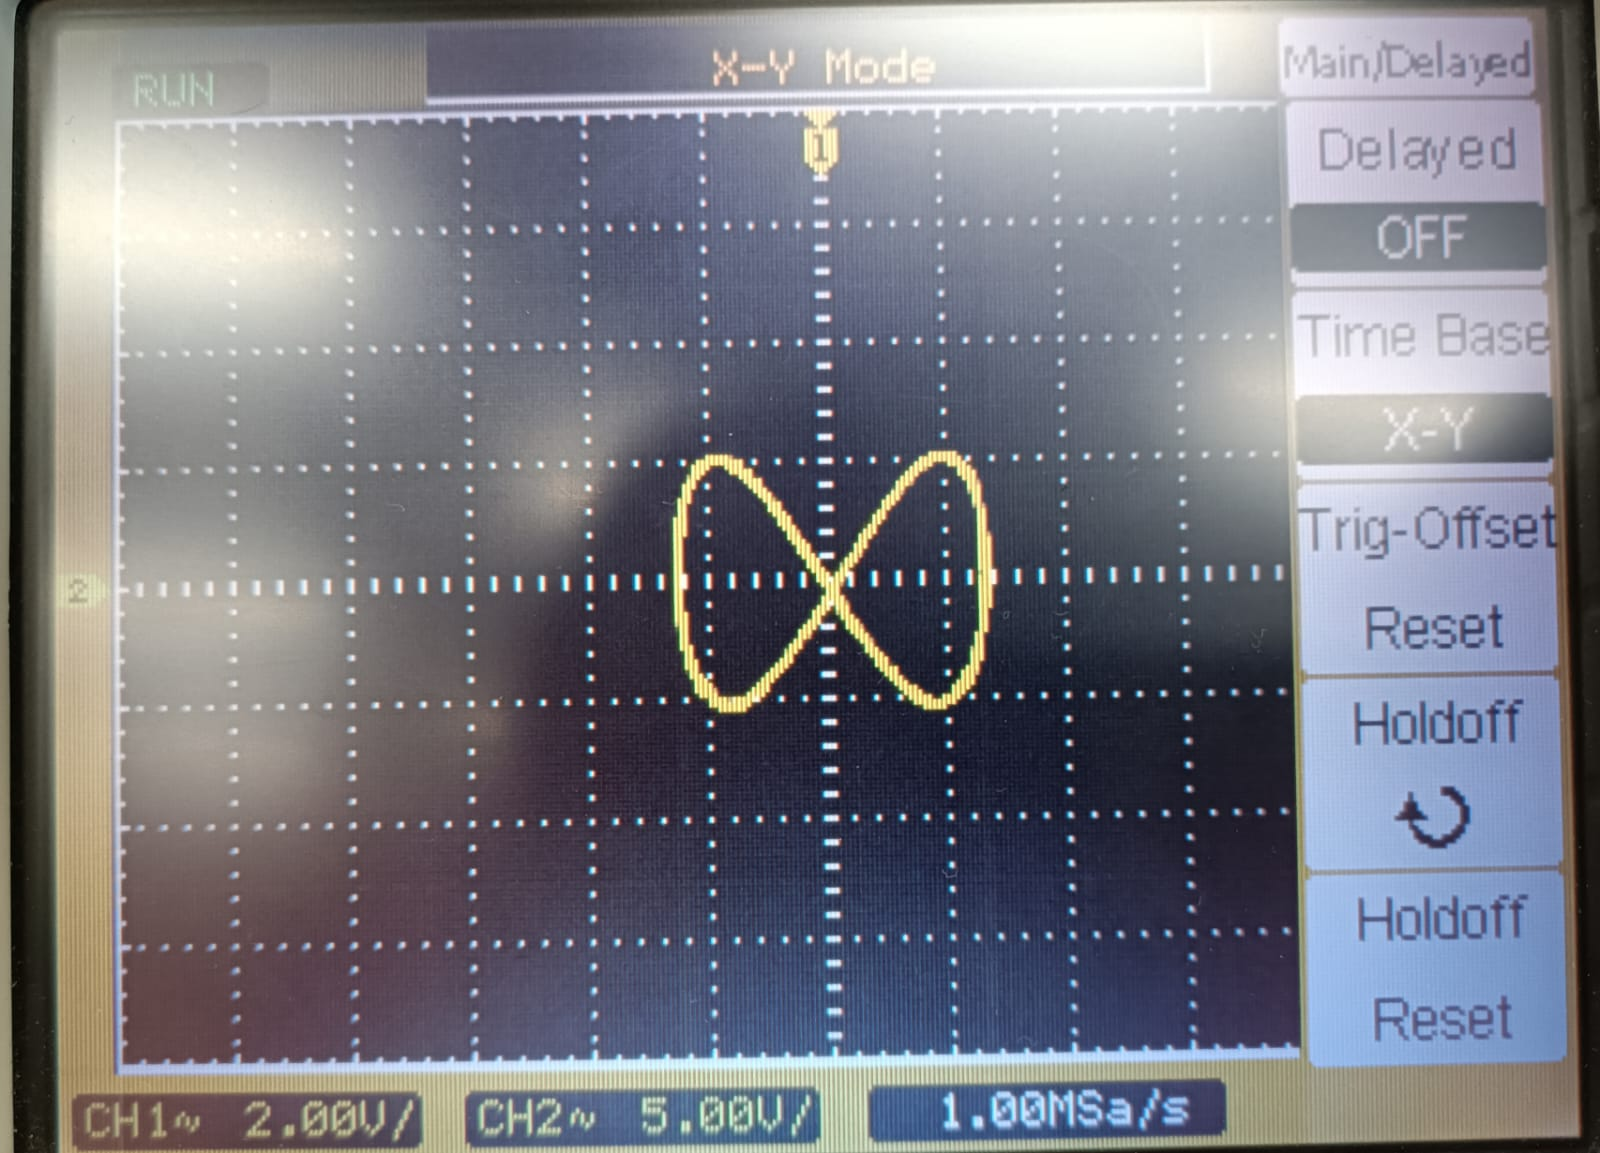
\includegraphics[width=0.6\textwidth]{actualgraph/infin.jpeg}
\caption{Graph of the above signal using Oscilloscope}
\label{fig:sample_image}
\end{figure}\\
Mathematical proof,\\
1. Using the trigonometric identity for \( \sin(2\theta) \):
\[
\sin(2\omega t) = 2 \sin(\omega t) \cos(\omega t),
\]
we substitute into \( y \):
\[
y = A_0 \cdot 2 \sin(\omega t) \cos(\omega t).
\]
\[
y = 2 A_0 \cos(\omega t) \cdot \sin(\omega t).
\]

2. From \( x = A_0 \sin(\omega t) \), solve for \( \sin(\omega t) \):
\[
\sin(\omega t) = \frac{x}{A_0}.
\]

3. Substitute \( \sin(\omega t) \) into the equation for \( y \):
\[
y = 2 A_0 \cos(\omega t) \cdot \frac{x}{A_0}.
\]
\[
y = 2 x \cos(\omega t).
\]

4. Use the Pythagorean identity \( \sin^2(\omega t) + \cos^2(\omega t) = 1 \) to solve for \( \cos(\omega t) \):
\[
\cos^2(\omega t) = 1 - \sin^2(\omega t).
\]
Substitute \( \sin(\omega t) = \frac{x}{A_0} \):
\[
\cos^2(\omega t) = 1 - \left(\frac{x}{A_0}\right)^2.
\]
\[
\cos(\omega t) = \pm\sqrt{1 - \frac{x^2}{A_0^2}}.
\]

5. Substitute \( \cos(\omega t) \) back into \( y \):
\[
y = 2 x \cdot \pm\sqrt{1 - \frac{x^2}{A_0^2}}.
\]


\begin{figure}[h!]
    \centering
    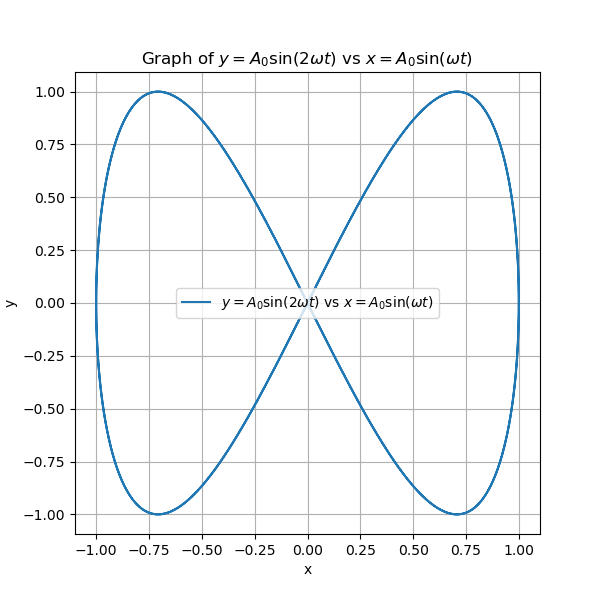
\includegraphics[width=0.3\textwidth]{graphs/Figure_3.png}
    \caption{Graph of the above signal using Python code}
    \label{fig:sample_image}
\end{figure}







\newpage
\item \textbf{\large \textbf{$x = A_0 \sin(\omega t)$} and \textbf{$y = A_0 \sin(3\omega t)$}}\\
 \begin{figure}[h!]
    \centering
    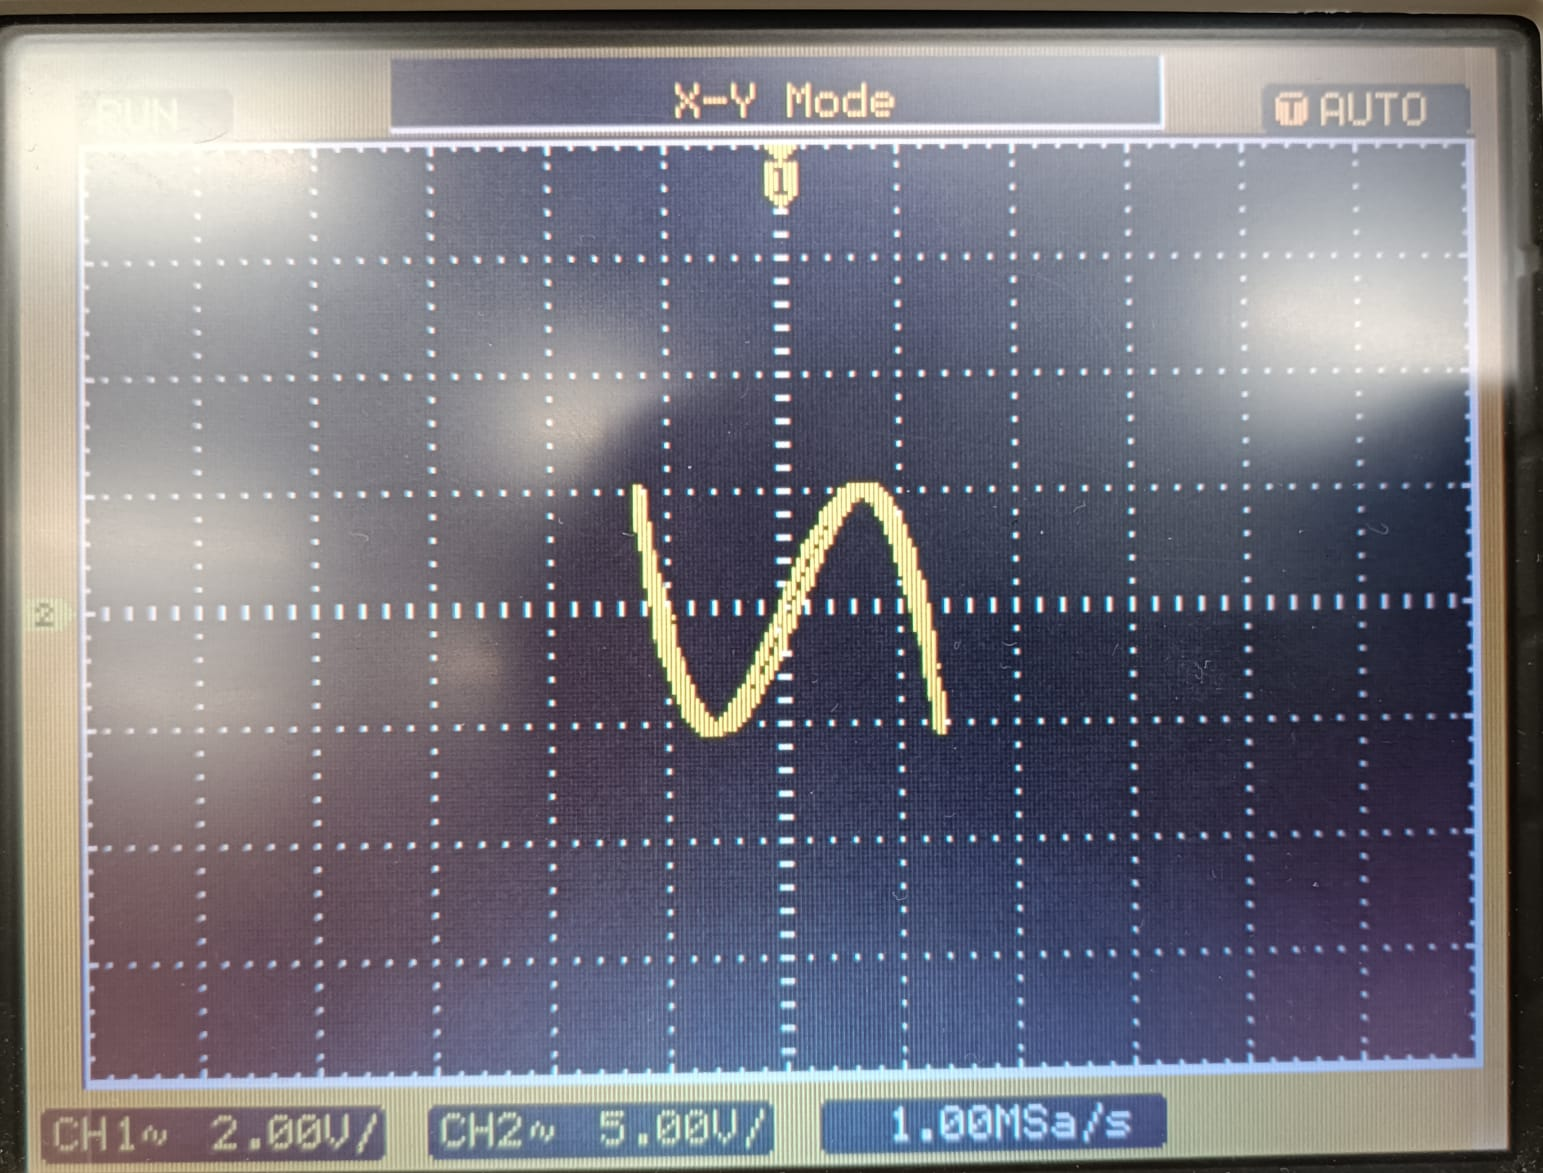
\includegraphics[width=0.3\textwidth]{actualgraph/3sin.jpeg}
    \caption{Graph of above signal in oscilloscope}
    \label{fig:sample_image}
    \end{figure}
Using the trigonometric identity for \(\sin(3\theta)\):
\[
\sin(3\omega t) = 3\sin(\omega t) - 4\sin^3(\omega t),
\]

we substitute \(\sin(\omega t) = \frac{x}{A_0}\) (from \(x = A_0 \sin(\omega t)\)) into \(y = A_0 \sin(3\omega t)\):
\[
y = A_0 \left[3\sin(\omega t) - 4\sin^3(\omega t)\right]
\]
\[
y = A_0 \left[3\frac{x}{A_0} - 4\left(\frac{x}{A_0}\right)^3\right]
\]

Simplify:
\[
y = 3x - \frac{4x^3}{A_0^2}.
\]

The final relationship is:
\[
y = 3x - \frac{4x^3}{A_0^2}.
\]
 \begin{figure}[h!]
    \centering
    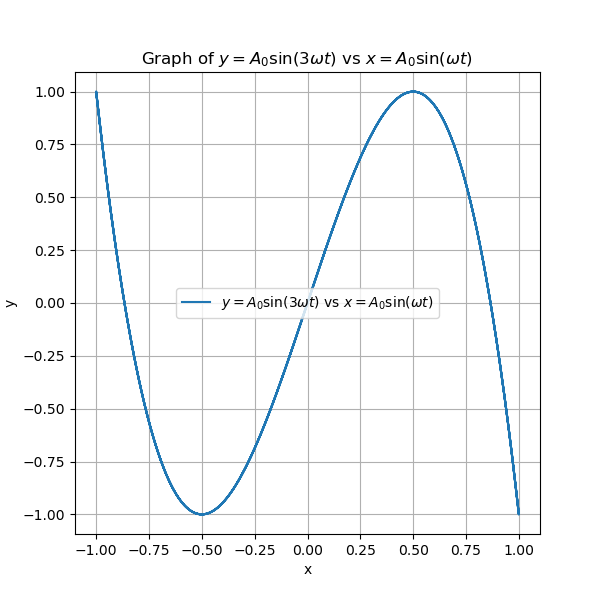
\includegraphics[width=0.3\textwidth]{graphs/Figure_4.png}
    \caption{Graph of above signal using python}
    \label{fig:sample_image}
     \end{figure}

\item \textbf{\large \textbf{$x = A_0 \sin(\omega t)$} and \textbf{$y = A_0 \sin(2\omega t+\frac{\pi}{2})$}},\\
\begin{figure}[h!]
    \centering
    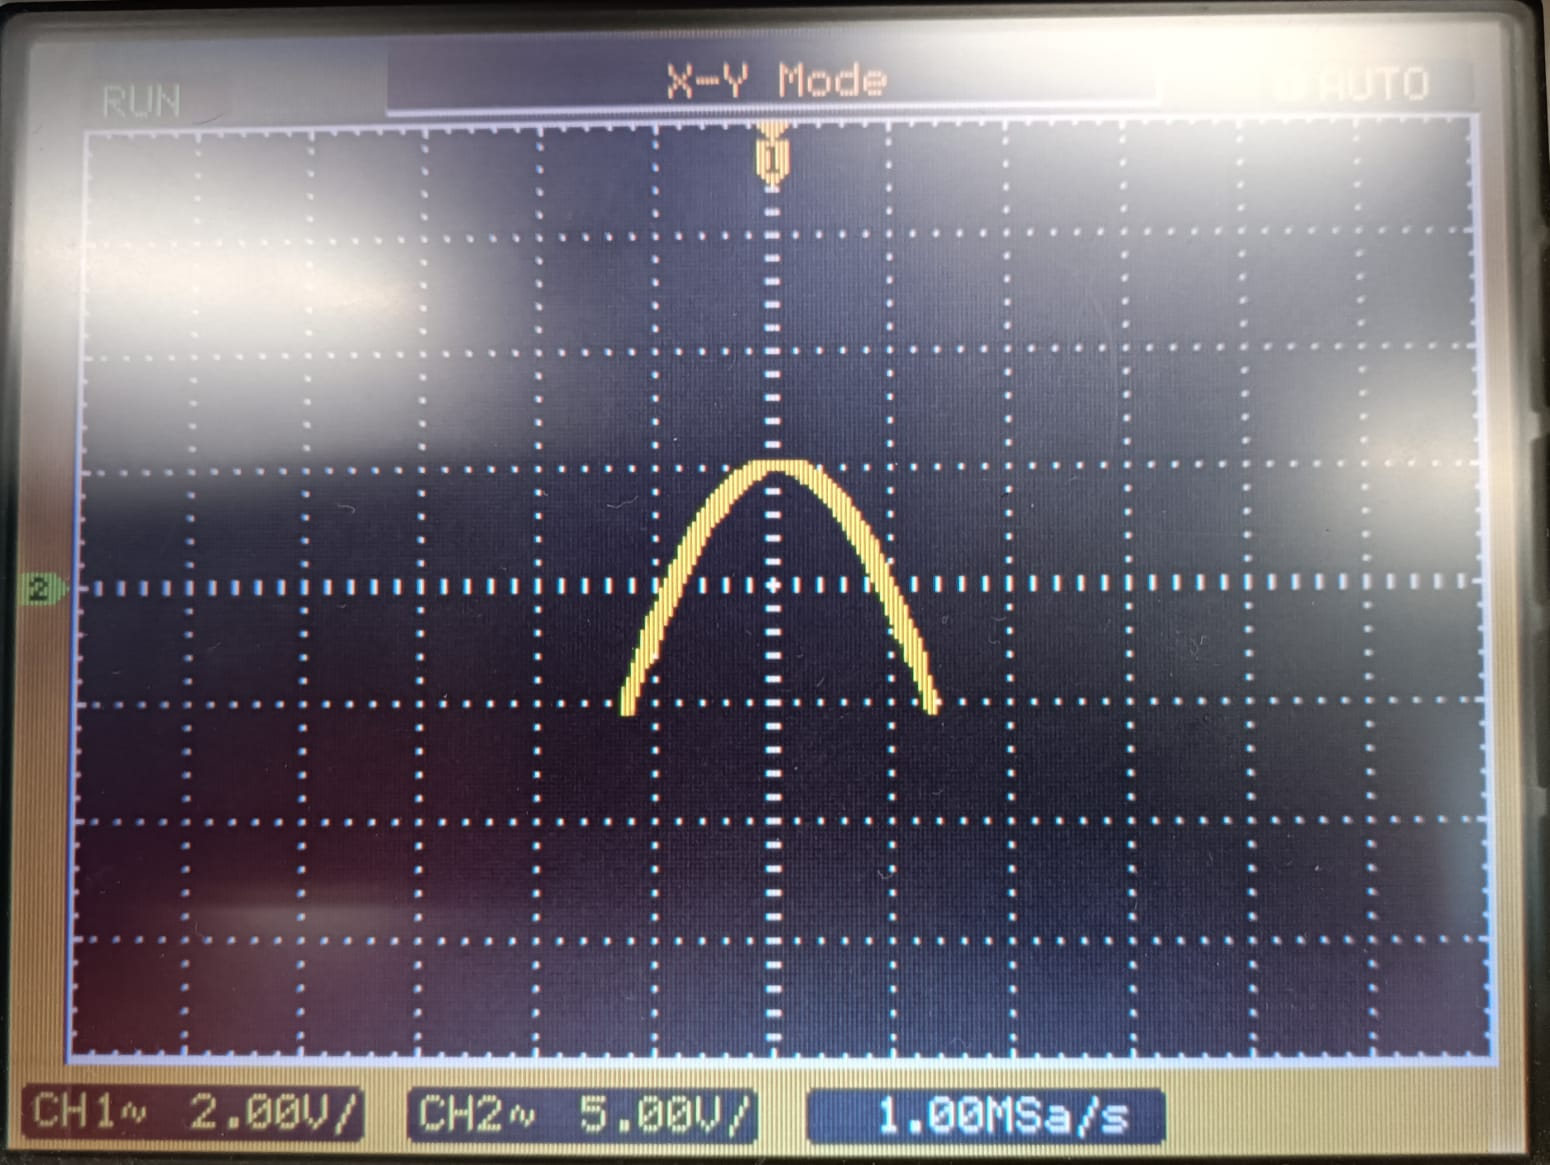
\includegraphics[width=0.6\textwidth]{actualgraph/parab.jpeg}
    \caption{Graph of above signal in oscilloscope}
    \label{fig:sample_image}
     \end{figure}

Mathematical proof,\\
\[
x = A_0 \sin(\omega t)\\
\]
\[
y = A_0 \sin(2\omega t+\frac{\pi}{2})\\
\]
\[
y= A_0 \cos(2\omega t)
\]
\[
y=A_0(1-2\sin^2(\omega t))
\]
\[
\implies y= A_0(1-2(\frac{x}{A_0})^2)
\]
Therefore, it is a parabola passing through y axis $A_0$
\begin{figure}[h!]
    \centering
    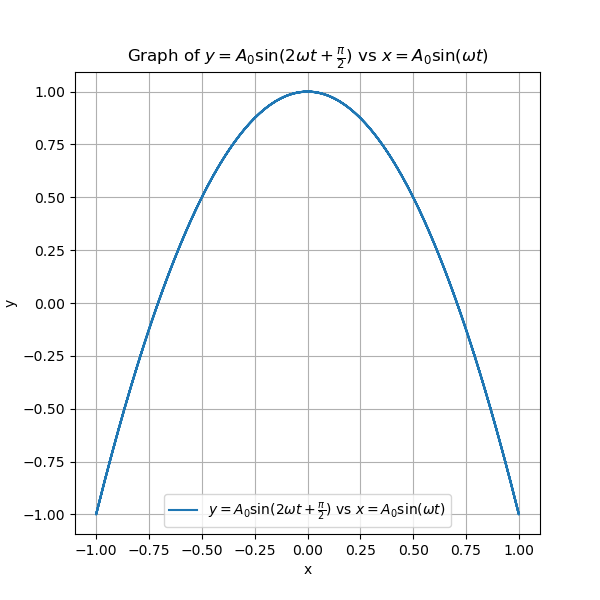
\includegraphics[width=0.4\textwidth]{graphs/Figure_5.png}
    \caption{Graph of above signal using python}
    \label{fig:sample_image}
     \end{figure}

\end{enumerate} 
\label{EndOfText}
\label{endOfDoc}
\newpage
\pagenumbering{arabic} 
\fancyfoot[C]{Page \thepage\ of \pageref{EndOfText}}
\section{One-time capture } \label{ch1}
\noindent1.The one-time capture feature on an oscilloscope allows you to capture and display a single, non-repetitive event or waveform.\\ 2.Unlike regular oscilloscope operation, which continuously displays repeating signals, the one-time capture freezes the oscilloscope's display after it detects a specific event, such as a glitch or an unexpected signal, that occurs only once or very infrequently.\\3. This is especially useful for analyzing rare issues that may not happen again during testing.
4.In this mode, the oscilloscope uses its trigger settings to capture the exact moment the event occurs.\\5. Once triggered, the oscilloscope captures the waveform and stores it in its memory for further analysis.\\ 6.This feature helps engineers diagnose problems that are hard to reproduce, making it easier to investigate and troubleshoot transient or irregular signals.
\subsection{Steps in one time capture}
\begin{itemize}
    \item Set the mode of oscilloscope to \textbf{Burst} mode.
    \item Select the trigger option in Function Generator.
    \item Set the number of bursts i.e, Number of Cycles to be captured.
    \item Connect the probes.
    \item The Number of cycles we have selected will be displayed on the screen .
\end{itemize}
\subsection{Example of One-time capture}
Here is the example of One-time capture of a square wave in which we took 7 Cycles ,\\
 \begin{figure}[h!]
    \centering
    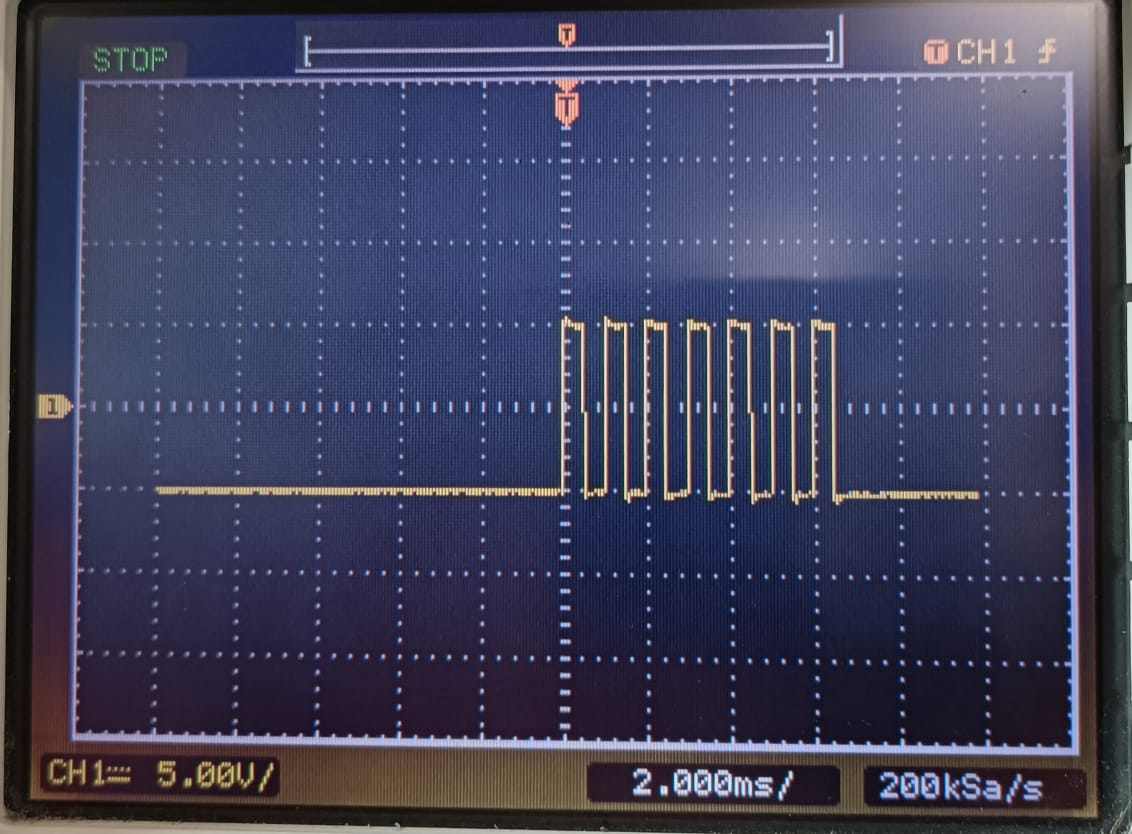
\includegraphics[width=0.45\textwidth]{actualgraph/7cycles.jpeg}
    \caption{Graph of above signal using python}
    \label{fig:sample_image}
     \end{figure}
     \newpage
Here is the picture of function generator related to above picture, \\
\begin{figure}[h!]
    \centering
    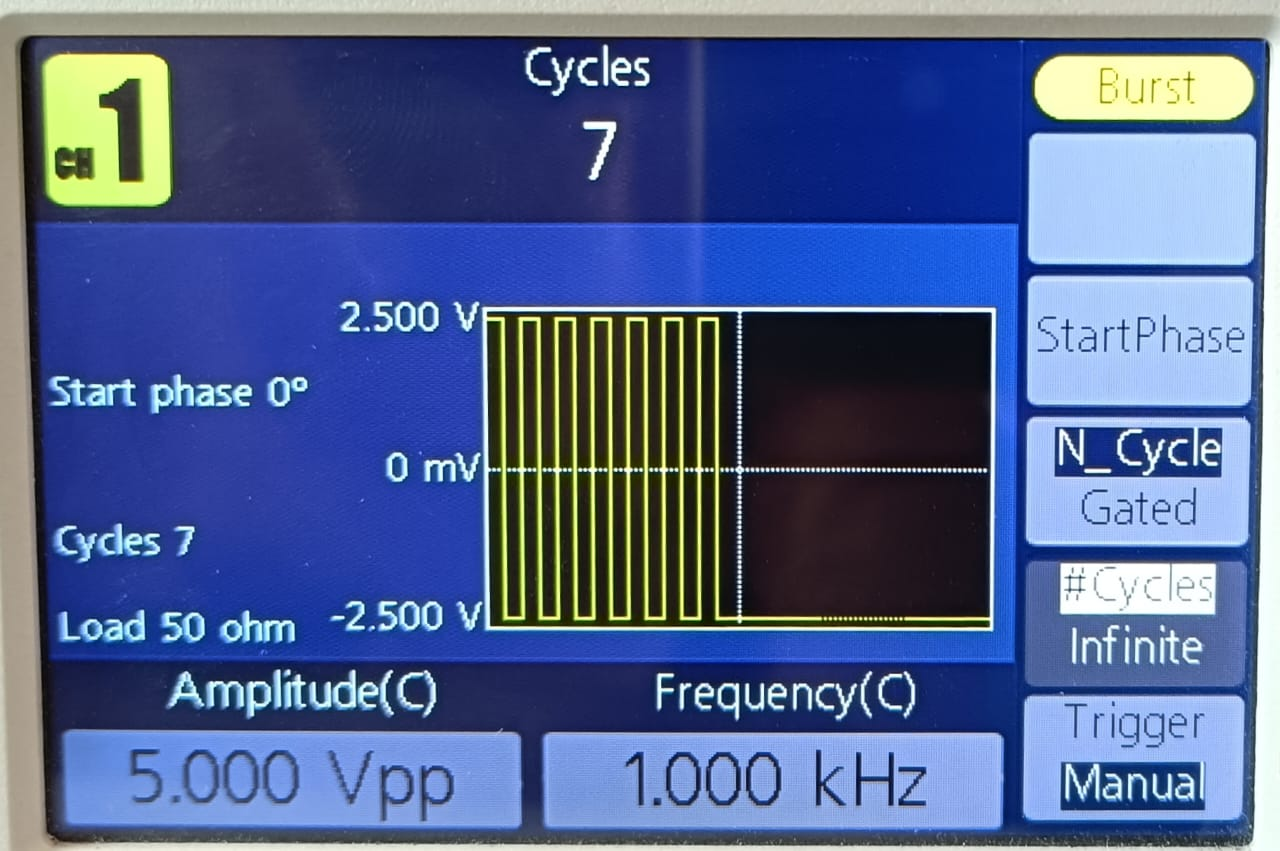
\includegraphics[width=0.6\textwidth]{actualgraph/funcgen.jpeg}
    \caption{Graph of above signal using python}
    \label{fig:sample_image}
     \end{figure}
 
\label{EndOfText}
\label{endOfDoc}
\newpage
\pagenumbering{arabic} 
\fancyfoot[C]{Page \thepage\ of \pageref{EndOfText}}
\section{References} \label{ch1}
\input{sources/references} 
\label{EndOfText}
\label{endOfDoc}
\end{document}
